\documentclass[a4paper]{report}
\usepackage[utf8]{inputenc}
\usepackage[T1]{fontenc}
\usepackage{RJournal}
\usepackage{amsmath,amssymb,array}
\usepackage{booktabs}
\usepackage{float}
\usepackage{xcolor}
\usepackage{ulem}
\usepackage{color}
\newcommand{\Y}[1]{{\color{blue}#1}}
\newcommand{\diag}[1]{\ensuremath{\mbox{diag}\left\{#1\right\}}}
%% load any required packages FOLLOWING this line
\newcommand{\stkout}[1]{\ifmmode\text{\sout{\ensuremath{#1}}}\else\sout{#1}\fi}
\begin{document}

%% do not edit, for illustration only
\sectionhead{Contributed research article}
\volume{14}
\volnumber{1}
\year{2022}
\month{March}
\setcounter{page}{212}

%% replace RJtemplate with your article
\begin{article}
  % !TeX root = RJwrapper.tex
\title{\pkg{starvars}: An R Package for Analysing Nonlinearities in Multivariate Time Series}
\author{by Andrea Bucci, Giulio Palomba and Eduardo Rossi}

\maketitle

\abstract{
Although linear autoregressive models are useful to practitioners in different fields, often a nonlinear specification would be more appropriate in time series analysis. In general, there are many alternative approaches to nonlinearity modelling, one consists in assuming multiple regimes. Among the possible specifications that account for regime changes in the multivariate framework, smooth transition models are the most general, since they nest both linear and threshold autoregressive models. This paper introduces the \CRANpkg{starvars} package which estimates and predicts the Vector Logistic Smooth Transition model in a very general setting which also includes predetermined variables. In comparison to the existing R packages,  \pkg{starvars} offers the estimation of the Vector Smooth Transition model both by maximum likelihood and nonlinear least squares. The package allows also to test for nonlinearity in a multivariate setting and detect the presence of common breaks. Furthermore, the package computes multi-step-ahead forecasts. Finally, an illustration with financial time series is provided to show its usage.
%This paper presents the \pkg{starvars} package which provides the tools for the estimation and prediction of a Vector Logistic Smooth Transition model. The user can choose among two estimation methods: maximum likelihood and nonlinear least squares. The package implements also some related functions that are useful to obtain and analyse time series of realized covariances, such as multivariate nonlinearity testing and common breaks detection.
}

\section{Introduction}

Many economic and financial time series often behave differently during stress periods for the economic activity. For example, during the subprime mortgage financial crisis, the relationship between the financial sector and macroeconomic quantities changed justifying the use of a nonlinear model. The same is also true in the analysis of monetary policy, where positive and negative monetary policy shocks may have asymmetric effects, or in the investigation of the effectiveness of a fiscal policy, where some fiscal policy measures may depend on the phase of the business cycle, see for example \cite{Caggiano2015}. When asymmetric effects are observed, the time series may follow different regimes. In order to understand the dynamics of such processes, \citet*{qua58, qua60} firstly proposed a model where the coefficients of a linear model change in relation to the value of an observable stochastic variable.  Afterwards, these models have been extended to time series analysis. \citet*{ton78} and \citet*{toli80} introduced the threshold autoregressive model, while \citet*{tera94} imagined that the transition between regimes could be smooth, which leads to the smooth transition autoregressive model (STAR) for univariate time series. 


Since researchers are often interested in understanding the dynamics of time series in a multivariate framework, regime-switching models have also been extended to include multiple dependent variables. A vector nonlinear model was introduced by \citet*{tsa98}, who defined a Threshold Vector Autoregressive (TVAR) model with a single threshold variable controlling the switching mechanism in each equation. The first vector model with a smooth transition was the smooth transition vector error-correction model (STVECM) introduced by \citet*{rovafra01}. In this model, the same transition function controls the transition in each equation. \citet*{cama:2004} proposed a bivariate logistic smooth transition model with the possibility to include exogenous regressors and specify a different transition variable for each equation. For a recent survey of vector TAR and STAR models, see \citet*{hute13}. More recently, \citet*{teraya14} presented a modelling strategy for building a Vector Logistic Smooth Transition Regression (VLSTAR). This strategy includes linearity and misspecification tests for the conditional mean, and testing the constancy of the error covariance matrix. 

This article summarizes the procedure proposed in \citet*{teraya14} and illustrates the \pkg{starvars} package in R for estimating and testing of the VLSTAR model with a single transition variable. Several packages for the estimation of the univariate logistic autoregressive model (LSTAR) are already present in R. For example, \citet*{tsdyn10} in their \CRANpkg{tsDyn} package provide functions to estimate and forecast both the STAR and the LSTAR models. Unfortunately, the \pkg{tsDyn} package, which focuses on nonlinear models in general, only allows for the estimation of a multivariate Threshold Vector Autoregressive (TVAR) model and does not allow for the inclusion of exogenous regressors. The \CRANpkg{RSTAR} package, implemented by \citet*{bal16}, estimates, forecasts, and analyses the smooth transition autoregressive model in the univariate case. Another possible way to model regime switches in a multivariate framework is through the \CRANpkg{MSBVAR} by \cite{MSBVAR}, capable of estimating a Markov-switching autoregressive model. Still, this package does not permit to evaluate the relationship between the dependent variables and possible explanatory variables.

The here presented R package \pkg{starvars} \citep{starvars20} is conceived for the nonlinear specification with a VLSTAR model of the relationship of multivariate time series exhibiting smooth nonlinear relationships with both their lags and a set of explanatory variables. Even though this model has been mainly applied in financial setups, it could be used in all fields in which the nature of the dynamics of the dependent variables could be conceived somehow nonlinear and, specifically, following a logistic smooth transition model. The functionalities of the \pkg{starvars} package include: (i) modelling strategy, such as joint linearity testing of multivariate time series, or detecting the presence of co-breaks, (ii) estimation and (iii) prediction of the VLSTAR model, (iv) construction of realized covariances from high and low-frequency financial prices or returns. Two datasets (\code{Realized} and \code{techprices}) are included in the R package \pkg{starvars}. The former entails monthly observations for realized co-volatilities between the S\&P 500, the Nikkei, the FTSE and the DAX indexes, the growth rate of the dividend yield and the earning price ratio, and the first difference of the inflation rate in the U.S., United Kingdom, Japan and Germany. The latter includes the data used in the example with the daily closing stock prices of Google, Microsoft and Amazon.

The outline of the paper is as follows. The following sections review the specification of the VLSTAR model, referring to \citet*{teraya14}, and illustrate how to estimate and make predictions through the \pkg{starvars} package. We then present an empirical application to stock price data, while the last section concludes.


\section{The Vector Logistic Smooth Transition Autoregressive Model} 
\label{Section2}

Assuming an $n \times 1$ vector of dependent time series, $y_t$, the multivariate smooth transition model introduced by \citet*{teraya14} can be written as follows
\begin{eqnarray}
\label{eq:VSTAR}
y_t & = & \mu_0+\sum_{j=1}^{p}\Phi_{0,j}\,y_{t-j}+A_0 x_t+
G_t\left(s_t;\gamma,c\right)\left[\mu_{1}+\sum_{j=1}^{p}\Phi_{1,j}\,y_{t-j}+A_1x_t\right]+\varepsilon_t\nonumber\\
& = & \mu_{0}+G_t\left(s_t;\gamma,c\right)\mu_{1}+\sum_{j=1}^{p}\left[\Phi_{0,j}+G_t\left(s_t;\gamma,c\right)\Phi_{1,j}\right]y_{t-j}
+\left[A_0+G_t\left(s_t;\gamma,c\right)A_1\right]x_t+\varepsilon_t,
\end{eqnarray}
where $\mu_{0}$ and $\mu_{1}$ are the $n \times 1$ vectors of intercepts, $\Phi_{0,j}$ and $\Phi_{1,j}$ are square
$n\times n$ matrices of parameters with lags $j=1,2,\dots,p$, $A_0$ and $A_1$ are $n\times k$ matrices of parameters,
$x_t$ is the $k \times 1$ vector of exogenous variables and $\varepsilon_t$ is the innovation. $G_t\left(s_t;\gamma,c\right)$ is a $n
\times n$ diagonal matrix of transition function at time $t$, such that
\begin{equation}
G_t\left(s_t;\gamma,c\right)=\diag{G_{1,t}\left(s_{1,t};\gamma_{1},c_{1}\right),G_{2,t}\left(s_{2,t};\gamma_{2},c_{2}\right),
	\dots,G_{n,t}\left(s_{n,t};\gamma_{n},c_{n}\right)},
\end{equation}
where $\gamma_i$ and $c_i$ are the scale and the threshold parameters for the $i$-th equation, for $i = 1, \ldots, n$.

In the VLSTAR model, each element of $G_t$ is specified as a logistic function
\begin{equation}
\label{eq:logistic}
G_{i,t}\left(s_{i,t}; \gamma_i, c_i\right) = \left[1 + \exp\big\{-\gamma_i\left(s_{i,t}-c_i\right)\big\}\right]^{-1}.
\end{equation}
Let $B=\left[G_t^{-1}\mu_0+\mu_1\quad G_t^{-1}\Phi_{0,1}+\Phi_{1,1}\quad G_t^{-1}\Phi_{0,2}+\Phi_{1,2}\quad\ldots\quad
G_t^{-1}\Phi_{0,p}+\Phi_{1,p}\quad G_t^{-1}A_0+A_1\right]'$, by reformulating Equation \eqref{eq:VSTAR} as in \cite{teraya14} and extending for the presence of $m$ regimes, Equation \eqref{eq:VSTAR} becomes


\begin{equation}
\label{eq:VLSTAR1}
y_t=\left\{\sum_{r=1}^m G_t^{r-1}B'_r\right\}z_t+\varepsilon_t=
\begin{bmatrix}I_{n} & G_t^1 & \ldots & G_t^{m-1}\end{bmatrix}
\begin{bmatrix}B_1\\B_2\\\vdots\\B_m\end{bmatrix}z_t+\varepsilon_t=\tilde{G}_t \tilde{B}'\,z_t+\varepsilon_t,
\end{equation}
where $\tilde{G}_t$ is a matrix of dimension $n\times m n$, $z_t=\left[1\quad y_{t-1}'\quad y_{t-2}' \quad\ldots\quad y_{t-p}'\quad x_t'\right]'$, $\tilde{B}$ is a $\left(1+k+p n\right)\times m n$ matrix and
$G_t^0=I_{n}$ is an identity matrix indicating that no transitions are allowed before the first change of regime. This equation defines the VLSTAR model with $m$ regimes and $p$ lags for the dependent variables.

The logistic function in Equation \eqref{eq:logistic} is accordingly modified as follows
\begin{equation}
\label{eq:transition}
G_{i,t}^r\left(s_{i,t}^r; \gamma_i^r, c_i^r\right) = \left[1 + \exp\big\{-\gamma_i^r(s_{i,t}^r-c_i^r)\big\}\right]^{-1},
\end{equation}
for $i = 1,2, \dots, n$ and $r=0,1,\dots,m-1$.



\subsection{Joint linearity test} \label{joint}

The VLSTAR specification procedure follows several steps. Firstly, the researcher should test whether the relationship between $y_t$ and $z_t$ can be linear. This is crucial, since several nonlinear models, like smooth transition and switching regression models, are not identified when the data-generating process is linear. With multivariate dependent variables, linearity can be tested equation by equation, using the Lagrange Multiplier (LM) test, as proposed by \citet*{lusate88}, \citet*{tera94} and \citet*{tetjg10}, or it may be tested simultaneously, as introduced by \citet{hute13} and \citet{teraya14b}.


The LM type statistic can be computed, as further suggested by \citet*{teraya14b}, using a multi-step procedure:
\begin{enumerate}
	\item estimation of the linear model, \textit{i.e.} the restricted VLSTAR with $\gamma = 0$;
	%the restricted model in Equation \eqref{eq:Taylor};
	\item save a collection of the residuals $(\tilde{\varepsilon}_t)$ from step 1 to create the residual matrix $\tilde{E}$ of dimension $T \times n$;
	\item computation of the residual sum of squares matrix, $Q = \tilde{E}'\tilde{E}$;
	\item regression of $\tilde{E}$ on $X$ and $V = \left(v_1', \ldots, v_T'\right)'$, where $v_t = \left(z_t's_t, z_t's_t^2, \ldots,  z_t's_t^d\right)$ and $s_t^d$ is the $d$-th order Taylor expansion of the logistic function (in our package $d = 3$, \textit{i.e.} a third-order Taylor expansion has been used);
	\item creation of the residual matrix, $\tilde{\Xi}$, from step 4 and the residual sum of square matrix, $\tilde{\Xi}'\tilde{\Xi}$;
	\item computation of the test statistic
	\begin{equation}\label{eq:LM2}
		LM = T \left\{Q^{-1}Q-\tilde{\Xi}'\tilde{\Xi}\right\} = T\left(p - tr\left\{Q^{-1}\tilde{\Xi}'\tilde{\Xi}\right\}\right) \sim \chi^2_{d n(np+1)}.
	\end{equation}
where $tr\{\cdot\}$ is the trace of the matrix.
	%Note that Equation \eqref{eq:LM2} is asymptotically equivalent to Equation \eqref{eq:LM1}.
\end{enumerate}

In the R package \pkg{starvars}, the joint linearity test can be performed by using the function \code{VLSTARjoint}, which takes the following arguments.
\begin{itemize}
	\item \code{y}: a \code{data.frame} or \code{matrix} containing the $T$ observations for the $n$ time series whose linearity should be tested;
	\item \code{exo}: an optional argument containing a \code{data.frame} or \code{matrix} of $k$ explanatory variables;
	\item \code{st}: a vector with the observations of the single transition variable $\left(s_t\right)$, or a matrix with a set of potential transition variables;
	\item \code{st.choice}: when the choice of the transition variable among a set of candidates should be based on the linearity test, this argument should be set equal to \code{TRUE}. In such a case, the variable in the matrix \code{st} which results in a higher LM statistics is the one chosen as the transition variable;
	\item \code{alpha}: a decimal value comprised between 0 and 1 ($\alpha \in [0,1]$) representing the confidence level, set to 0.05 by default.
\end{itemize}

In this case, the residuals $\tilde{\varepsilon}_t$ used in step 2 of the above-mentioned procedure are obtained through a VAR($p$) estimation of the restricted model in step 1. This is done through the \code{VAR} function from R package \CRANpkg{vars}, with an automatically selected number of lags, $p$. 
%
\begin{example}
	VLSTARjoint(y, exo, st, st.choice = FALSE, alpha = 0.05)
\end{example}
%
The function \code{VLSTARjoint} returns a list object with a class attribute \code{"VLSTARjoint"}, for which \code{print} method exists, with three elements: the value(s) of the Lagrange Multiplier value (LM), the $p$-value(s) of the test and the critical value. 

Furthermore, the specification of the VLSTAR model foresees the definition of the number of regimes to be used in the model (see Appendix A for further details). The function \code{multiCUMSUM} allows determining the number of common breaks and where they are located. 
%
\begin{example}
	multiCUMSUM(data, conf.level = 0.95, max.breaks = 7)
\end{example}
%
The arguments necessary to detect the common breaks are: a matrix of $T \times n$ of time series, in the argument \code{data}; the confidence level in \code{conf.level}, set by default at 0.95; the number of maximum common breaks (between 1 and 7) to be identified, through \code{max.breaks}. The output is returned in a list with a class attribute \code{"multiCUMSUM"}, which can be passed through the \code{print} function. The first element of the returned list object is a matrix with the test statistics $\Lambda_T$ and $\Omega_T$ (see Equation \eqref{eq:lambda} in Appendix A for details). The list further reports the index of the common breaks detected and the correspondent dates, as long as the critical values for both $\Lambda_T$ and $\Omega_T$.

\subsection{VLSTAR Estimation}

As widely discussed in \citet*{teraya14}, a VLSTAR model can be estimated through a nonlinear Least Square (NLS) or a maximum likelihood (ML) model. 

In both cases, the optimization algorithm may converge to some local minima, attributing to the definition of valid starting values of the estimated parameters a special relevance. If there is no clear indication of the initial values of $\gamma$ and $c$, this can be done by implementing a grid search. Thus, a discrete grid in the parameter space is created to obtain the estimates of $B$ conditionally on each point in the grid. The initial pairs of $\gamma$ and $c$ producing the smallest sum of squared residuals are chosen as initial values. A pair of these parameters for each equation is selected unless common parameters are assumed. Given their values, the model is linear in parameters.

The searching grid algorithm works as follows:
\begin{enumerate}
	\item construction of the grid for $\gamma$ and $c$, computing the vector of parameters for each point in the grid;
	\item estimation of $\tilde{B}$ in each equation through NLS and computation of the residual sum of squares, $Q$;
	\item find the pairs of $\gamma$ and $c$ providing the smallest $Q$ which will be the starting $\gamma_0$ and $c_0$;
	\item estimation of parameters, $\tilde{B}$, via NLS or ML;
	\item estimation of $\gamma$ and $c$ for each equation given the parameters found in step 4;
	\item repeat steps 4 and 5 until convergence.
\end{enumerate}

The \pkg{starvars} package allows the user to implement a searching grid algorithm to obtain the initial values of $c$ and $\gamma$. Specifically, the practitioner may obtain initial values through the \code{startingVLSTAR} function among a set of potential values. For example, by providing \code{n.combi}$=50$, $50$ values of $\gamma$ and $c$ are combined in a grid of $2500$ couples of values as in step 1 of the former procedure. The values of the grid for $\gamma$ range from 0 to 100, while the values of $c$ range from minimum to maximum of each dependent variable.

The \code{startingVLSTAR} function requires several arguments. A \code{data.frame} or a \code{matrix} of dimension $T \times n$ containing the dependent variables of the model, representing \code{y}. An optional argument,  \code{exo}, contains possible explanatory variables and can be specified as a \code{data.frame} or a \code{matrix} with the same length of \code{y} and $k$ columns. The lag-order $p$ should be specified as an integer. The number of regimes in the model is set by the argument \code{m}, while the transition variable $s_t$ of length $T$ is specified in the argument \code{st}. The number of cores used to make parallel computation is specified through the \code{ncores} argument, while the argument \code{singlecgamma} works as follows:
		\begin{itemize}
			\item \code{singlecgamma = TRUE}: it is assumed a common pair of initial values for the entire model;
			\item \code{singlecgamma = FALSE}: a pair of $c$ and $\gamma$ is obtained for each of the equations.
		\end{itemize}
%
\begin{example}
	startingVLSTAR(y, exo = NULL, p = 1,
	m = 2, st = NULL, constant = TRUE,
	n.combi = NULL, ncores = 2,
	singlecgamma = FALSE)
\end{example}
%


\subsubsection{VLSTAR Estimation via NLS}
The NLS estimator is defined as the solution to the following optimisation problem
\begin{equation}\label{eq:minQT}
\hat{\theta}_{NLS} = \underset{\theta}{\arg\min}\sum_{t=1}^{T}\left(y_t-\tilde{G}_t\tilde{B}'z_t\right)'\left(y_t-\tilde{G}_t\tilde{B}'z_t\right)
\end{equation}
where $\theta$ is the set of parameters to be estimated.

In the aforementioned algorithm, the vectorization of the NLS estimates of $\tilde{B}$ for step 4, given the values of $\gamma$ and $c$, is equal to:
\begin{equation}\label{eq:NLS}
\text{vec}(\tilde{B})_{NLS} = \left[T^{-1}\sum_{t=1}^{T}\left(\tilde{G}_t \tilde{G}'_t\right)\otimes \left(z_t z_t'\right)\right]^{-1} \left[T^{-1}\sum_{t=1}^{T}\text{vec}\left(z_t y_t' \tilde{G}'_t\right)\right].
\end{equation}
The estimated errors covariance matrix is given by
\begin{equation}\label{eq:Omega}
\hat{\Omega}_{NLS} = T^{-1}\hat{E}'\hat{E},
\end{equation}
where $\hat{E} = \left(\hat{\varepsilon}_1, \ldots, \hat{\varepsilon}_n\right)'$ is a $T \times n$ matrix, and $\hat{\varepsilon}_t = y_t - \tilde{G}_t\tilde{B}_{NLS}'z_t$ is a column vector of residuals. This is used to obtain the first iterative ML estimation in the previous algorithm in step 4.


\subsubsection{VLSTAR Estimation via ML}
To estimate a VLSTAR model via ML, it must be assumed that $\varepsilon_t\sim i.i.d.N(0,\Omega)$. In this case, the model can be represented by the following multivariate conditional density function
\begin{equation}\label{eq:ML}
f\left(y_t|\mathcal{I}_T;\theta\right)=\left(2\pi\right)^{-\frac{n}{2}}|\Omega|^{-\frac{1}{2}}\exp\left\{-\frac{1}{2}\left(y_t-\tilde{G}_t\tilde{B}'\,z_t\right)'\Omega^{-1}\left(y_t-\tilde{G}_t\tilde{B}'\,z_t\right)\right\},
\end{equation}
where $\mathcal{I}_t$ is the information set at time $t$ which contains all the exogenous variables $x_t$ and all the lags of $y_t$. 

In the first iteration of the algorithm presented in this section, $\Omega$ is estimated through Equation \eqref{eq:Omega}. Consequently, the ML estimator of $\theta$ is obtained by solving the optimization problem
\begin{equation}
\hat{\theta}_{ML} = arg \max_{\theta}\ell\left(y_t|\mathcal{I}_t;\theta\right).
\end{equation}


\subsection{Estimation in the starvars package} \label{estimationR}



In the \pkg{starvars} package, the estimation of a VLSTAR model is handled with the function \code{VLSTAR}. By fitting such a model via this function, a list object with a class attribute \code{"VLSTAR"} is obtained. This function requires the same arguments of the \code{startingVLSTAR} function, except for the number of combinations. In addition, a \code{list} of \code{data.frame} or \code{matrix} containing starting values of $c$ and $\gamma$, for each of the $m-1$ logistic functions as in Equation \eqref{eq:transition}, must be passed through the argument \code{starting}. The user can choose the method used to estimate the coefficients among the `ML' and the `NLS' through the specification of the argument \code{method}. The argument \code{epsilon} is used as a convergence check while the argument \code{ncores} denotes the number of cores used in the parallel optimization of the objective function.

%
\begin{example}
	VLSTAR(y, exo = NULL, p = 1, m = 2, st = NULL, constant = TRUE,
	starting = NULL,
	method = c('ML', 'NLS'), 
	n.iter = 500, singlecgamma = TRUE, 
	epsilon = 10^(-3), ncores = NULL)
\end{example}
%


The \code{summary} method applied to an object derived from the \code{VLSTAR} function returns the sample size, along with the number of estimated parameters, the multivariate log-likelihood calculated as in Equation \eqref{eq:ML},
and the estimated coefficients. We also provide other generic methods, such as \code{plot}, \code{AIC}, \code{BIC} and \code{logLok}. Similar to what is implemented in the R package \pkg{vars}, the \code{plot} function reports for each equation in the VLSTAR model the observed values of each time series, the fitted values and the residuals, as well as the autocorrelation and partial autocorrelation functions of the residuals. Since the logistic function plays a crucial role in VLSTAR models, the \code{plot} function shows also the plot of the logistic function for each dependent variable. 


\subsection{Forecasting a VLSTAR model}\label{Sub24}
Time series prediction using nonlinear models has become widespread in the last few decades, even if the debate on the usefulness of such forecasts is still open \citep[see][]{dienaso1990, kote11}. The forecasts of the nonlinear model, for more than one step ahead, can be generalised via numerical techniques. Given a nonlinear model
\begin{equation}
y_t = g\left(z_t,\theta\right) + \varepsilon_t,
\end{equation}
where $\theta$ is a vector of parameters to be estimated, $z_t$ is a combination of lagged values of $y_t$ and exogenous variables $x_t$, and $\varepsilon_t$ is a white noise with zero mean and constant variance $\sigma^{2}$, the forecast of $y_{t+h}$ made at time $t$ is equal to the conditional mean
\begin{equation}
\label{eq:nlinearforecast}
\hat{y}_{t+h\mid t}=E\left\{y_{t+h}| \mathcal{I}_t\right\}=E\left\{g(z_{t+h-1})|\mathcal{I}_t\right\}.
\end{equation}
where $\mathcal{I}_t$ is the information set at time $t$ and	$\varepsilon_t$ is independent of $\mathcal{I}_{t-1}$.

When $h=1$, the forecast $\hat{y}_{t+1}=g(z_t)$ is obtained from Equation \eqref{eq:nlinearforecast}; if $h \geq 2$, the
prediction can only be calculated recursively using numerical techniques. 

The nonlinearity in the VLSTAR model makes multi-period forecasting more complicated. In fact, forecasting two steps ahead is not straightforward, since we have
\begin{equation}\label{eq:tplus2}
y_{t+2| t} = E\left(y_{t+2}| \mathcal{I}_t\right) = E\left\{\big[g(z_{t+2};\theta)+\varepsilon_{t+2} \big]| \mathcal{I}_t\right\}
\end{equation}
and consequently
\begin{equation}
y_{t+2\mid t} = E\left\{\big[g(z_{t+2};\theta)+\varepsilon_{t+2} \big]| \mathcal{I}_t\right\}=\int_{-\infty}^{+\infty}g(z_{t+2}\theta)d\Phi(v)dv
\end{equation}
where $\Phi(v)$ is the cumulative distribution function for $\varepsilon_{t+1}$. It follows that to obtain the $t+2$ forecast of $y$ numerical integration would be necessary, while multiple integrations would be required for longer time horizons; see \citet*{lute07}. 
 

The R package \pkg{starvars} can handle both one-step and multi-step-ahead forecasts of an object with a class attribute \code{"VLSTAR"}. One-step-ahead forecasts can be easily extended to the multivariate framework by modifying Equation \eqref{eq:VLSTAR1} as follows
\begin{equation*}
	y_{t+1} = \tilde{G}_{t+1}\left(s_{t+1}; \hat{\gamma}, \hat{c}\right) \hat{\tilde{B}}' z_{t+1}
\end{equation*}
where $\hat{\tilde{B}}$ is the matrix of estimated parameters and $z_{t+1} = \left[1, y_{t}', y_{t-1}', \ldots, y_{t-p+1}', x_{t+1}'\right]'$, while $\tilde{G}_{t+1}$ is calculated using estimated values of $\gamma$ and $c$. Multi-step-ahead forecasts are slightly trickier to be found and several alternatives can be used. As shown in \citet*{lute07} for the univariate case, multi-step-ahead forecasts can be obtained in three ways: naively, by Monte Carlo simulation and by bootstrapping. The method \code{predict} in the \pkg{starvars} package allows the user to choose between these methods through the argument \code{method}. When the \code{naive} method is chosen, the $y_{t+h}$ forecasts are obtained as follows
\begin{equation*}
	y_{t+h}^{na} = \tilde{G}_{t+h}\left(s_{t+h}; \hat{\gamma}, \hat{c}\right) \hat{\tilde{B}}' z_{t+h}^{na}
\end{equation*}
where $z_{t+h}^{na} = \left[1, y_{t+h-1}', \ldots, y_{t+h-p}', x_{t+h}'\right]'$. If the transition variable is the lagged $y_{t-s}$, with $s < h$, the prediction of the $i$-th element of $y$ is used as a new transition variable, otherwise the new value of $s_t$ should be passed through the argument \code{st.new}. The index $i$ is specified by the argument \code{st.num}, which denotes the column number of the dependent variable which should be used as a new transition variable. From \citet{hute13}, \citet{kote11} and \citet{tetjg10}, we know that these forecasts are biased. Thus, the practitioner may choose the \code{Monte Carlo} method. In this case, $\varepsilon_{t+1}$ should be simulated using a properly defined error distribution. Let $\hat{B}_1 = \left[\hat{\mu}_0, \hat{\Phi}_{0,1}, \ldots \hat{\Phi}_{0,p}, \hat{A}_0\right]$ and $\hat{B}_2 = \left[\hat{\mu}_1, \hat{\Phi}_{1,1}, \ldots, \hat{\Phi}_{1,p}, \hat{A}_1\right]$, the multivariate version of the Monte Carlo method for $h$ steps ahead is given by
\begin{equation*}
	y_{t+h}^{mc} = \hat{B}_1'z_{t+h} + \frac{1}{M}\sum_{m=1}^{M} \tilde{G}_{t+h}\left(s_{t+h}; \hat{\gamma}, 
	\hat{c}\right)\hat{B}_2'z_{t+h}^{mc}
\end{equation*}
where $z_{t+h}^{mc} = \left[1, \left(y_{t+h-1}+\varepsilon_{t+h}^{mc}\right)', \ldots, \left(y_{t+h-p}+\varepsilon_{t+h-p+1}^{mc}\right)', x_{t+h}'\right]'$,  $\varepsilon_{t+h}^{mc}$ is a vector of errors sampled from a Multivariate Normal distribution with zero mean and covariance matrix $\hat{\Omega}$. In such a case, the interval forecasts are directly determined from the forecast density. Finally, the \code{bootstrap} method foresees that the multi-step-ahead forecasts are derived from
\begin{equation*}
	y_{t+h}^{bo} = \hat{B}_1'z_{t+h} + \frac{1}{B}\sum_{b=1}^{B} \tilde{G}_{t+h}\left(s_{t+h}; \hat{\gamma}, \hat{c}\right)\hat{B}_2'z_{t+h}^{bo}
\end{equation*}
where $z_{t+h}^{bo} = \left[1, \left(y_{t+h-1}+\varepsilon_{t+h}^{bo}\right)', \ldots, \left(y_{t+h-p}+\varepsilon_{t+h-p+1}^{bo}\right)', x_{t+h}'\right]'$, $\varepsilon_{t+h}^{bo}$ is sampled from the $T \times n$ matrix of residuals. As in the case of the \code{Monte Carlo} method, the interval forecasts are derived from the forecast density.
%
\begin{example}
	predict(object, ..., n.ahead = 1, conf.lev = 0.95, st.new = NULL, 
	st.num = NULL, newdata = NULL, 
	method = c('naive', 'Monte Carlo', 'bootstrap'))
\end{example}
%
The \code{predict} method returns a list with a class attribute \code{"vlstarpred"} and two elements: a list denoted with the name \code{forecasts} containing the predicted values and the interval forecasts for each of the steps ahead, and the matrix with the values of $y$. The \code{print} method is applicable to objects of this class and returns the forecasts with upper and lower interval forecasts. The \code{plot} method draws the time series plots with the interval forecasts in the out-of-sample period.


\section{VLSTAR model compared to other linear and nonlinear models}
The here applied VLSTAR model is one of the possible ways of modelling nonlinear relationships. Alternatively, nonlinearity in a multivariate framework can be modelled through a Threshold Vector Autoregression (TVAR) or Markov-switching Vector Autoregressive (MSVAR) model. The VLSTAR and the TVAR models are both based on the assumption that the variable that defines the regime-switching is observable, while the MSVAR is mainly based on the assumption that regime-switches are defined by a latent Markov process. When the practitioner has enough information on the factors that drive the dynamics of the dependent variables, using VLSTAR or TVAR models may reduce the uncertainty related to the regimes and may produce more accurate predictions than an MSVAR model \cite[see][]{hute13}. In other words, the VLSTAR is a model with a continuum of states where the change between a number of regimes is smooth, the TVAR is mostly conceived to analyse the dynamics of variables that switch abruptly between the regimes. The VLSTAR model can be seen as a general version of the TVAR that allows also for the regimes to change smoothly. Indeed, when $\gamma \rightarrow \infty$ for each regime, the VLSTAR model becomes a TVAR model with well-defined changes of regimes. Conversely, when $\gamma \rightarrow 0$, the model becomes a simple VAR model.
	
The \pkg{starvars} package further differs from the \pkg{tsDyn} and the \pkg{MSBVAR} by \cite{MSBVAR} packages, which permit the estimation of the TVAR and MSVAR models, since it allows the use of exogenous variables in the estimation set. This is a useful tool since practitioners may control for potential explanatory variables different from lags of the dependent variable to obtain parameter estimates and dependent variables predictions.




\section{Example} \label{Section4}


To illustrate how the R package \pkg{starvars} works in practical situations, we present an empirical application with multivariate time series of stock prices. Starting from the prices of $n=3$ stocks of the tech companies, Amazon, Microsoft and Google, available in the dataset \code{techprices}, we model the monthly realized covariances assuming that their dynamics can be captured by a flexible specification like the VLSTAR model which nests the linear VAR. First, we construct the $n(n+1)/2$ monthly series of realized covariances and their Cholesky factors which are modelled through VLSTAR. This solves the problem of obtaining positive semidefinite covariance matrices that can be used in finding optimal portfolios. Second, from the estimated VLSTAR, we can compute the forecasts of the monthly realized covariances, see \cite{chivo11, buparo19, buc20jf}.
In particular, asset returns co-volatilities tend to be higher when bad news is available. From Figure \ref{fig:Figure0}, it is clearly observable that co-volatilities explode during periods of market turmoil, like the subprime mortgage crisis in 2007 or the spread of the COronaVIrus Disease 19 (COVID-19) at the beginning of 2020. This explains why co-volatilities exhibit nonlinear behaviour.


\begin{figure}[H]
	\centering
	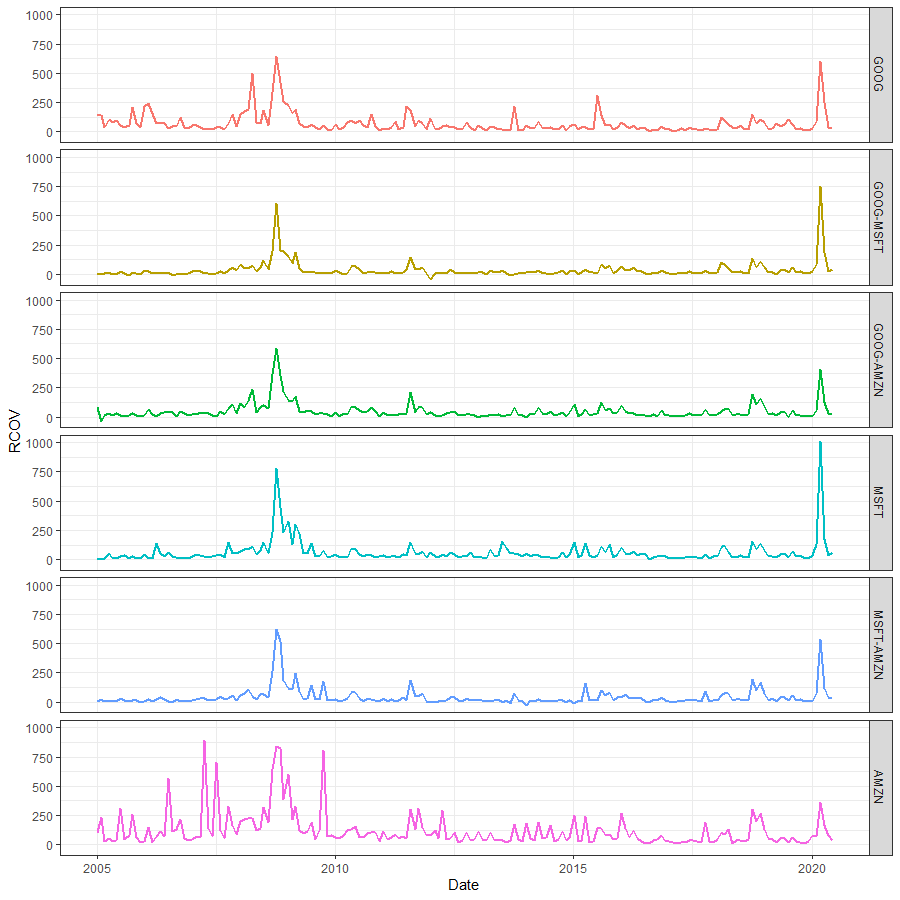
\includegraphics[width = \columnwidth]{Nonlinear}
	\caption{\label{fig:Figure0} Plots of realized covariances of the stock returns. The panels report the realized variances (one stock symbol, \textit{i.e.} first, third and last panel) and covariances (two symbols, \textit{i.e.} second, third and fifth panel) between the considered stocks. `GOOG' is the stock symbol of Google, `MSFT' is the stock symbol of Microsoft, and `AMZN' is the stock symbol of Amazon. The time series show several peaks during periods of financial market stress such as the sub-prime mortgage crisis and the COVID-19 pandemic in 2021, which may underline a nonlinear behaviour of co-volatilities.}
\end{figure}

 The \code{techprices} dataset used in this example includes the closing prices from January 1st 2005 to June 16th 2020, for a total of 3,890 observations per series. The dataset can be loaded in the workspace using

%
\begin{example}
> data("techprices", package = "starvars")
\end{example}
%
where \code{techprices} is a $3,890 \times 3$ \code{xts} object containing the daily prices. As a first step, we calculate the realized covariances of stock returns and their Cholesky factors. Since we have already daily prices, we can only build monthly, quarterly, or yearly realized covariances. To keep the sample of realized covariances quite large, we calculate monthly realized covariances and their Cholesky factors through the code (further discussed in Appendix B):
%%We then subset \code{techprices} to select just the prices of Amazon and Google.
%
%\begin{example}
%> techprices <- techprices[,1:2]
%\end{example}
\begin{example}
> RCOV <- rcov(techprices, freq = "monthly", make.ret = TRUE, cholesky = TRUE)
\end{example}
%
from which we obtain a list of two elements in the object \code{RCOV}. We are just interested in the Cholesky factors of the stock returns, thus we save the desired \code{data.frame} in the object \code{techchol} with a class \code{"xts"}.
%
\begin{example}
> techchol <- RCOV$'Cholesky Factors'
\end{example}
%
which has dimension $T \times n(n+1)/2$, where $T = 186$ and $n(n+1)/2 = 6$. Therefore, in our example there are $n(n+1)/2 = 6$ dependent variables.
		
The modelling strategy of a VLSTAR model starts with a test for the time series nonlinearities. As largely explained above, this can be done via the \code{VLSTARjoint} function. Since no information about which variable should be used as a transition variable is available, we let the linearity test choose among a set of potential variables which are equal to the first lag of the dependent variables. The LM statistics and the related $p$-value for a given value of \code{alpha} (set equal to 0.05 by default) and for the chosen transition variable can be obtained simply by running
%
\begin{example}

> st <- lag(techchol,1)[-1]
> VLSTARjoint(techchol[-1,], st = st, st.choice = TRUE)

Joint linearity test (Third-order Taylor expansion)
Transition variable chosen: y5 
LM = 158.7 ; p-value = 2.0595e-21 
Critical value for alpha = 40.646

\end{example}
%	
		
The linearity test indicates the presence of nonlinearity in the data, and that the rejection of the null hypothesis is stronger when the lag of the fifth Cholesky factor, \code{y5}, is chosen as the transition variable. At this point, the practitioner should assess the presence of common breaks among the time series through the test presented in Appendix A. The test, for a maximum number of breaks equal to 3, is computed as follows.
		
%
\begin{example}
> multiCUMSUM(techchol[-1], max.breaks = 3)
============================================================
Break detection in the covariance structure:
Lambda Omega Break Date 1 Break Date 2 Break Date 3
Break 1  11.10  3.93   2009-04-03                          
Break 2  21.53  9.64   2009-04-03   2007-12-03             
Break 3  12.09  6.03   2009-04-03   2007-12-03   2015-07-03
============================================================
Critical values are 2.69 for Lambda and 1.74 for Omega.
2 Break(s) identified with Lambda 
2 Break(s) identified with Omega
\end{example}
%	
This function returns significant test statistics for all the breaks for $\Lambda_T$ and $\Omega_T$, which both identify a number of breaks equal to 2. To keep the model parsimonious, we decide to include a single break and $m=2$ regimes in our example.
		
Given that a nonlinear model would be necessary and that at least a single break is present in the multivariate time series, a VLSTAR model can be estimated. Before estimating the parameters, we implement the searching grid algorithm to find starting values of $\gamma$ and $c$ with 20 potential values each (400 combinations). Specifying \code{singlecgamma = FALSE} we are supposing that each equation has its own parameters. Once executed the code, a progress bar is shown to inform the user about the completion of the searching grid algorithm.

%
\begin{example}
>  starting <- startingVLSTAR(techchol[-1,], p = 1, m = 2, st = st[,5], 
+		n.combi = 20, singlecgamma = FALSE, ncores = 4)
\end{example}
%	
We employ an NLS estimation, with the lag of the fifth Cholesky factor as $s_t$, a single lag $p=1$, two regimes $m=2$, a number of maximum iterations equal to 30 and a number of cores for parallel computation equal to 4, and we use the starting values found in the previous step of the procedure saved in the \code{starting} object. Therefore, we show the code used to specify the VLSTAR model as well as the summary output, and the graphic for the equation of the first Cholesky factor, \code{y1}.

\begin{example}
>  fit.VLSTAR <- VLSTAR(techchol[-1,], p = 1, m = 2, st = st[,5],
+	method = 'NLS', starting = starting, n.iter = 30, ncores = 4)
> summary(fit.VLSTAR)
> plot(fit.VLSTAR, names = "y1")
Model VLSTAR with 2 regimes
Full sample size: 184 
Number of estimated parameters: 108 	Multivariate log-likelihood: 2272.663 
==================================================

Equation y1 

Coefficients regime 1 
const        y1        y2        y3        y4        y5        y6 
8.108***    0.038     0.135     0.123     0.142  -1.379***    0.330  

Coefficients regime 2 
const        y1        y2        y3        y4        y5        y6 
10.613***  0.411***   -0.067   0.593*** -1.884***   0.669**  1.762*** 

Gamma: 3.0809 	c: 3.1603 
AIC: 769.78 	BIC: 814.79 	LL: -370.89 

Equation y2 

Coefficients regime 1 
const      y1      y2      y3      y4      y5      y6 
0.511  -0.019   0.106  0.250**  0.126  -0.005   0.261  

Coefficients regime 2 
const        y1        y2        y3        y4        y5        y6 
6.919***  0.760***   -0.136     0.177* -0.644*** -1.688***  0.613*** 

Gamma: 866.3921 	c: 3.5162 
AIC: 545.65 	BIC: 590.66 	LL: -258.83 

Equation y3 

Coefficients regime 1 
const       y1       y2       y3       y4       y5       y6 
1.015*  -0.033    0.053  0.389***   0.003    0.022    0.295  

Coefficients regime 2 
const        y1        y2        y3        y4        y5        y6 
-3.503***  1.419***   -0.123     0.218* -0.580*** -0.895***   -0.425* 

Gamma: 110.8034 	c: 3.595 
AIC: 571.67 	BIC: 616.67 	LL: -271.83 

Equation y4 

Coefficients regime 1 
const        y1        y2        y3        y4        y5        y6 
4.270***   -0.034    -0.046     0.058    0.340** -1.114***    0.096  

Coefficients regime 2 
const        y1        y2        y3        y4        y5        y6 
11.561***   0.127**    0.166.  0.287*** -0.939*** -0.497***  1.117*** 

Gamma: 1.1841 	c: 3.4705 
AIC: 496.2 	BIC: 541.21 	LL: -234.1 

Equation y5 

Coefficients regime 1 
const      y1      y2      y3      y4      y5      y6 
0.367  -0.009   0.061   0.096. -0.012  0.200**  0.158  

Coefficients regime 2 
const        y1        y2        y3        y4        y5        y6 
7.756*** -0.695*** -0.337***  0.290*** -0.418***  0.639***  1.269*** 

Gamma: 100 	c: 4.1137 
AIC: 351.31 	BIC: 396.32 	LL: -161.66 

Equation y6 

Coefficients regime 1 
const        y1        y2        y3        y4        y5        y6 
2.693***   -0.005     0.005     0.048     0.120. -0.234***    0.171. 

Coefficients regime 2 
const        y1        y2        y3        y4        y5        y6 
3.648***  0.383***   -0.138*  0.199*** -0.992***   0.178**  0.909*** 

Gamma: 69.405 	c: 3.5824 
AIC: 324.3 	BIC: 369.31 	LL: -148.15 
==================================================

Signif. codes:  0 '***' 0.001 '**' 0.01 '*' 0.05 '.' 0.1 ' ' 1 
\end{example}
		%
		
After the execution of the code, a counter with the number of the iteration in the estimation algorithm is shown until convergence or the maximum number of iterations is reached. Using a laptop with an Intel\textsuperscript{\textregistered} Core\texttrademark i5-7200U 2.5GHz processor with 16 GB RAM, the searching grid algorithm takes around 40 seconds to find optimal values of $\gamma$ and $c$, while convergence is achieved after 7 iterations taking around 500 seconds (with the package version 1.1.10). The estimation process could take from a few minutes to several hours depending on the complexity of the model. The number of parameters increases with the number of dependent variables, the number of exogenous variables, and the number of regimes, therefore affecting the optimization problem and the convergence time. For example, the estimation of the former example with $m=3$ regimes takes about an hour and 30 minutes.
		
The results of the \code{plot} function on the Equation of \code{y1} in the \code{VLSTAR} object are shown in Figure \ref{fig:Figure1}. It may be noticed from the last panel of the Figure reporting the logistic function that the assumption of a smoothing regime-switching is realistic. 
		
		
		
\begin{figure}[ht!]
			\centering
			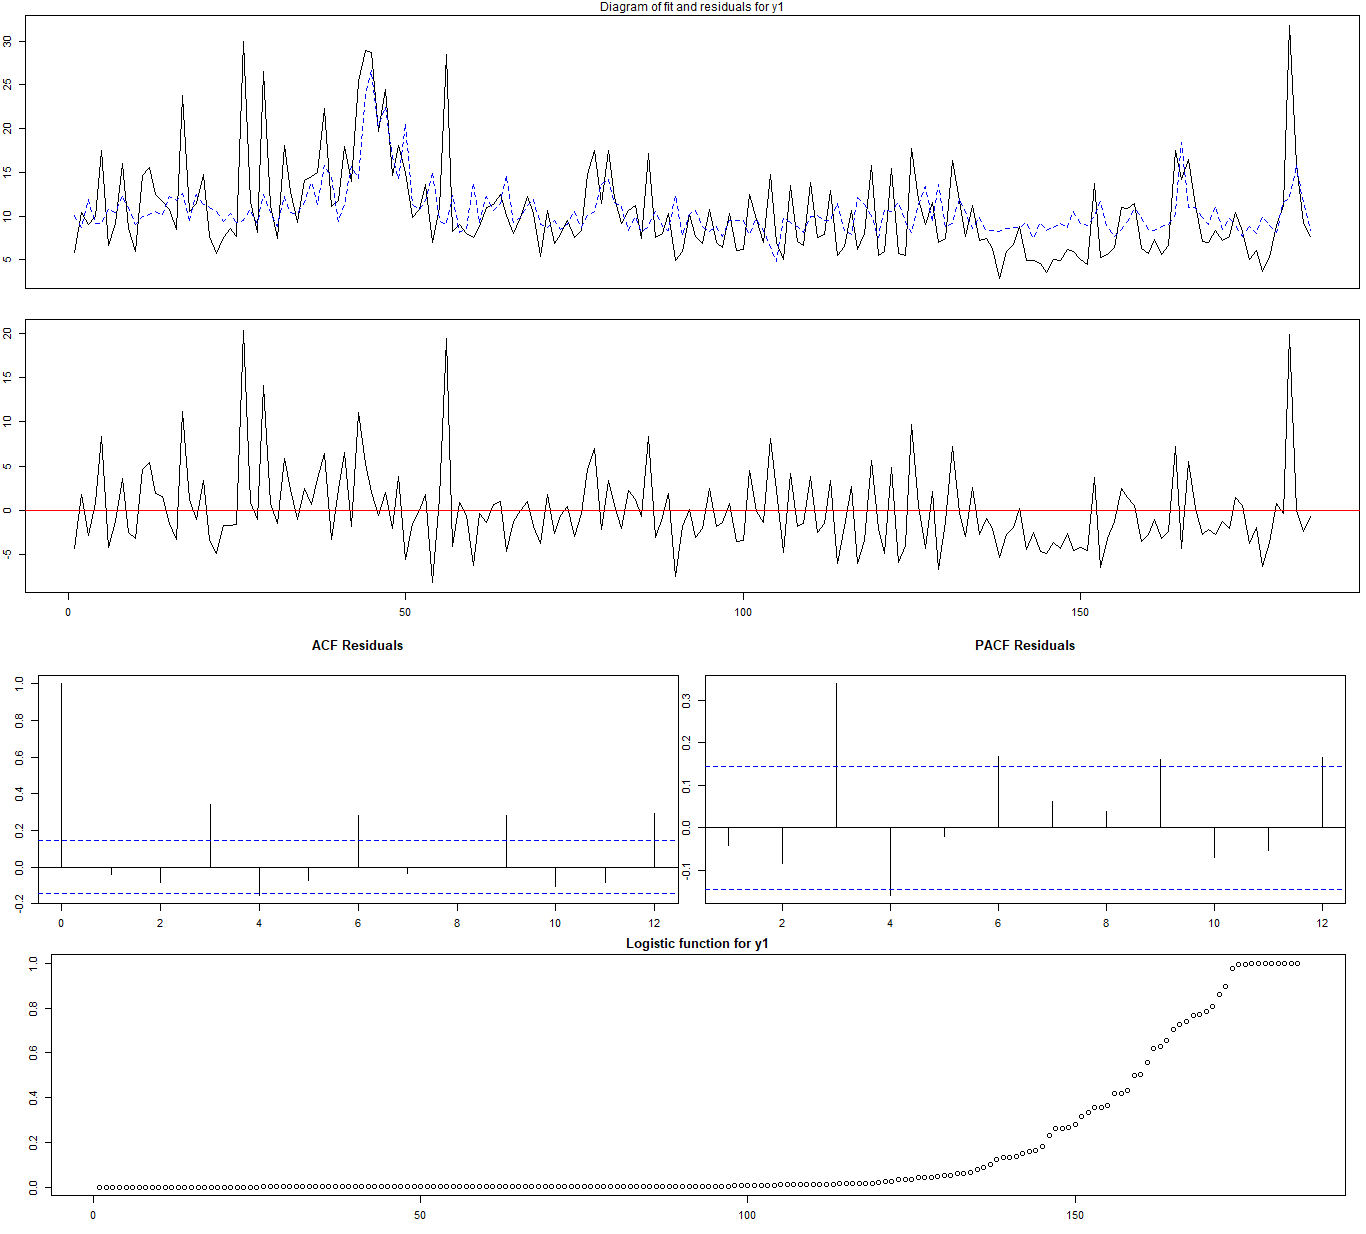
\includegraphics[width = \columnwidth]{Equationy1}
			\caption{\label{fig:Figure1} Plots of results from VLSTAR estimation for the Equation of \code{y1}. The first panel shows the observed time series (in black) versus the fitted time series (in dashed blue). The second panel shows the residuals and highlights the zero with a red horizontal line. The left side of the third panel reports the autocorrelation function of the residuals, while the right side reports the partial autocorrelation function of the residuals. The fourth panel is about the logistic function that regulates the regime switches. The residual time series of $y1$ seems to show poor autocorrelation, while the regime switches appear to be quite smooth.}
\end{figure}
\clearpage
		
		
Time series models are usually implemented to make out-of-sample predictions. In our package, this is possible through the \code{predict} method that, applied to objects of class \code{"VLSTAR"}, returns an object with a class \code{"vlstarpred"}. When using the \code{predict} function, the argument \code{method = 'bootstrap'} specifies that the aforementioned ``bootstrap'' method has been used to make predictions, while the argument \code{n.ahead = 2} denotes that two-step-ahead predictions are obtained. The outcome of the \code{plot} method of the out-of-sample forecasts for the first Cholesky factor is exhibited in Figure \ref{fig:Figure2}. The predictions of the Cholesky factors could be used to obtain a semidefinite positive predicted covariance matrix by simply inverting the Cholesky decomposition.

		
		
%
\begin{example}
> pred.bootstrap <- predict(fit.VLSTAR, n.ahead = 2, st.num = 5, method = 'bootstrap')
> pred.bootstrap
$y1
		   fcst lower 95% upper 95%
Step 1  8.370493  7.283483  9.457503
Step 2 20.916559 12.878648 28.649321

$y2
		   fcst lower 95% upper 95%
Step 1 3.131276  2.540087  3.722465
Step 2 6.188201  4.761677  7.948755

$y3
		   fcst lower 95% upper 95%
Step 1 3.508982  2.874487  4.143478
Step 2 6.631187  4.822495  9.018994

$y4
		   fcst lower 95% upper 95%
Step 1  5.188099  4.671238   5.70496
Step 2 12.483377  8.961486  15.73787

$y5
		   fcst lower 95% upper 95%
Step 1 1.794161  1.445520  2.142802
Step 2 3.293723  2.469695  4.301613

$y6
		   fcst lower 95% upper 95%
Step 1 3.381696  3.057729  3.705664
Step 2 7.258409  6.307594  8.322091
\end{example}
%
				
%
\begin{example}

> plot(pred.bootstrap, type = 'single', names = 'y1')

\end{example}
%
				
				
\begin{figure}[H]
					\centering
					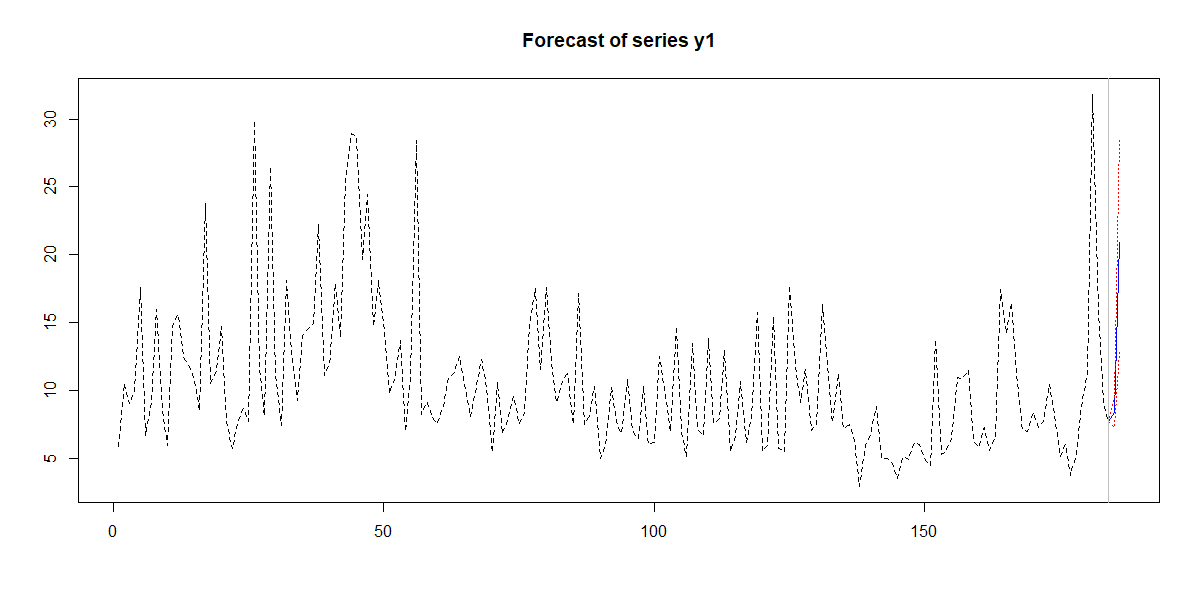
\includegraphics[width = \columnwidth]{pred.bootstrap}
					\caption{\label{fig:Figure2} Out-of-sample predictions of time series \code{y1}. The plot shows the observed time series in-sample (in dashed black), the two-step ahead out-of-sample predictions (in dashed blue), and their 95\% prediction interval (in dashed red). A vertical grey line denotes the end of the in-sample observations. The predictions of time series $y1$ highlight that the prediction interval is extremely tight and that predictions can be nonlinear.}
\end{figure}
				
				
\section{Conclusion} \label{Section5}

This article introduces the R package \pkg{starvars} for modelling, estimating, and forecasting a Vector Logistic Smooth Transition Autoregressive (VLSTAR) model. We present the model specification in a general way and illustrate the package usage. In particular, we perform an empirical application using financial data.

The package allows practitioners in many scientific areas to perform their applied research using VLSTAR models in a user-friendly environment. The build-in framework permits to analyse nonlinearity of time series and make multi-step-ahead predictions via different methods. Further, the practitioner may use the \pkg{starvars} package to obtain realized covariances at several frequencies and the Cholesky decomposition of the related realized covariance matrices.

It should be reminded that the estimation of the parameters in a VLSTAR model strongly depends on the initial values of the parameter of the logistic. We have observed that sometimes the algorithm underlying the automatic grid search may lead to unrealistic estimates of the logistic parameters and, consequently, to not consistent estimates of coefficients. Moreover, the computational time, when using more than two regimes, might be compromised by a large number of coefficients and a possible local minimum may be found by the maximization of the log-likelihood. Thus, the suggestion is to use a limited number of regimes to keep the model as parsimonious as possible.

The code of the package \pkg{starvars} may be improved by using a different transition variable for each equation or by allowing the estimates of a univariate model. However, in both cases, the estimation would be reduced to a univariate model for each equation and there are already packages able to do this. 

				
\section{Availability}
The here presented package is written using S4 classes and provides methodology such as \code{coef}, \code{plot}, \code{AIC}, \code{BIC}, \code{logLik}, \code{summary} and \code{print} to analyze the results. The R package \pkg{starvars} is available from the Comprehensive R Archive Network (CRAN) at \url{https://cran.r-project.org/package=starvars} and on GitHub at \url{https://github.com/andbucci/starvars}.

\newpage
\bibliography{starvars}

\newpage
\section{Appendix A: Testing for common breaks}\label{common}

If the linearity hypothesis is rejected, the researcher should determine the number of regimes of the dependent variable. To this end, the procedure introduced by \citet*{baipe98,baipe03} may be implemented. In presence of multivariate time series, it may happen that sudden shocks, such as market crashes, financial crises, or interventions of policymakers, result in a structural break in the mean of the observed time series \citep[see][]{stock1998}. At the same time, the interest of the researcher may be directed to changes in the structure of the conditional correlations \citep[see][]{bara2020, aue2009}. To detect the presence of structural breaks in the co-movements of the $n$ time series, \citet*{aue2009} introduced a test on the structure of the covariances. Here, we attempt to summarize the procedure\footnote{See the original paper by \citet*{aue2009} for the technical details.}.

Let $\left(y_t: t\in \mathbb{Z}\right)$ be a sequence of $n$ time series, with $E[y_t] = \mu$ and $E[| y_t|^2] < \infty$, where $\mid \cdot \mid$ denotes the Euclidean norm in $\Re^n$, then the null hypothesis in a test for structural breaks in the co-volatilities process is given by
\begin{equation*}
	H_0\colon Cov(y_1) = \ldots = Cov(y_T)
\end{equation*}
where $T$ is the number of observations. This means that the covariances are constant over the observed period. A common alternative hypothesis would be that there is at least one change in the covariance structure which corresponds to the presence of at least one common break.

Provided that $E[y_t] = 0$, the test statistic is based on the constancy of the expected values $E[vech(y_t y_t')]$ for $t = 1, \ldots, T$ under $H_0$. As a consequence, from the estimates of $E[vech(y_t y_t')]$ on $j$ observations (with $j < T$), a traditional cumulative sum (CUSUM) statistic can be constructed as
\begin{equation}
	S_j = \frac{1}{\sqrt{T}}\Bigg(\sum_{t=1}^j vech[y_t y_t']-\frac{j}{T}\sum_{t=1}^{T}vech[y_t y_t']\Bigg), \text{with } j = 1, \ldots, T.
\end{equation}
Let $\tilde{y}_t = y_t - \overline{y}_T$, where $\displaystyle\overline{y}_T = \frac{1}{T}\sum_{t=1}^T y_t$, if the zero mean assumption does not hold, \textit{i.e.} $E[y_t] \neq 0$, then $S_j$ can be replaced by
\begin{equation}
	\tilde{S}_j = \frac{1}{\sqrt{T}}\Bigg(\sum_{t=1}^j vech[\tilde{y}_t \tilde{y}_t']-\frac{j}{T}\sum_{t=1}^{T}vech[\tilde{y}_t \tilde{y}_t']\Bigg), \text{with } j = 1, \ldots, T.
\end{equation}
Given the long-run covariance estimator $\hat{\Sigma}_T$, the test statistics are
\begin{equation}\label{eq:lambda}
	\Lambda_T = \underset{1 \leq j \leq T}{\max} S_j' \hat{\Sigma}_T^{-1}S_j \text{ and } \Omega_T = \frac{1}{T}\sum_{j=1}^T S_j' \hat{\Sigma}_T^{-1}S_j
\end{equation}
as well as
\begin{equation*}
	\tilde{\Lambda}_T = \underset{1 \leq j \leq T}{\max} \tilde{S}_j' \hat{\Sigma}_T^{-1}\tilde{S}_j \text{ and } \tilde{\Omega}_T = \frac{1}{T}\sum_{j=1}^T \tilde{S}_j' \hat{\Sigma}_T^{-1}\tilde{S}_j.
\end{equation*}
For the critical values of these statistics, it should be referred to \citet*{aue2009}.

Once the null hypothesis can be rejected, the researcher should find the location of both the breakpoint and the breakpoint fraction $\theta$ whose estimation is given by
\begin{equation}
	\hat{\theta}= \frac{1}{T} \underset{1 \leq j \leq T}{\arg\max} S_j' \hat{\Sigma}_T^{-1}S_j.
\end{equation}
This can be repeated for each partition of the entire sample to obtain the optimal number and location of common breaks. On the basis of what is found with the test on common breaks, the number of regimes of the VLSTAR model can be assessed and parameters estimation can be performed.

\section{Appendix B: Realized covariances construction} \label{Section32}

Along with the specification of a VLSTAR model, the R package \pkg{starvars} allows the user to calculate a non-parametric measure of volatility in the multivariate framework, such as the realized volatility \citep[see][for the theoretical fundamentals]{abde01, abdl03, bash02}. Given a vector of stock returns, $r_\tau$ sampled at a given frequency, $\tau$, the realized covariance matrix, $RC_t$ observed at a lower frequency $t$ is simply given by
\begin{equation}
	RC_t = \sum_{\tau=1}^{N_t}r_{\tau}r_{\tau}'
\end{equation}
where $N_t$ is the number of observations in the $t$-th period and $t = 1,\ldots, T$. 

The function \code{rcov} in the package \pkg{starvars} returns the lower triangular of $RC_t$ starting both from stock prices or returns, and to calculate it for different frequencies. 
%
\begin{example}
	rcov(data, freq = c('daily', 'monthly', 'quarterly', 'yearly'), 
	make.ret = TRUE, cholesky = FALSE)
\end{example}
%
The function consists of several arguments. An object of class \code{"xts"} with the values of stock prices or returns on which the realized covariances should be calculated. The frequency of $t$, which could be \code{daily}, \code{monthly}, \code{quarterly} or \code{yearly}. The boolean argument \code{make.ret} denotes whether the data passed as input in the argument \code{data} should be converted to returns, if \code{TRUE} the returns are calculated. Finally, since a wide strand of the literature relies on the Cholesky factors of $RC_t$ to make inference or predictions \citep*[see][for example]{beclo10, chivo11, buparo19, buc20jf}, the function also allows the user to calculate the Cholesky factors, $L_t$, such that 
\begin{equation*}
	RC_t = L_tL_t'.
\end{equation*}
This can be done by setting the argument \code{cholesky} equal to \code{TRUE}. If \code{make.ret} is set equal to \code{TRUE}, the output of the function \code{rcov} contains an element of class \code{"xts"} with the returns.

When \code{cholesky = TRUE}, the output of the \code{rcov} function is a list containing the $T\times n(n+1)/2$ \code{xts} object from the vectorization of the realized covariance matrices, given by $vech(RC_t)$, and the $T\times n(n+1)/2$ of the vectorization of $L_t$, given by $vech(L_t)$, otherwise it includes only the series of realized covariances.

\newpage
\address{Andrea Bucci\\
  Department of Economics, Universit\`a degli Studi G. d'Annunzio Chieti-Pescara\\
  Viale Pindaro 42, Pescara\\
  Italy\\
  https://orcid.org/0000-0001-9872-9761\\
  \email{andrea.bucci@unich.it}}

\address{Giulio Palomba\\
  Department of Economics and Social Sciences, Universit\`a Politecnica delle Marche\\
  Piazzale Martelli 8, Ancona\\
  Italy\\
  \email{g.palomba@staff.univpm.it}}

\address{Eduardo Rossi\\
  Department of Economics and Management, University of Pavia\\
  Via S. Felice Al Monastero 7, Pavia\\
  Italy\\
  https://orcid.org/0000-0003-3597-8060\\
  \email{eduros04@unipv.it}}

\end{article}

\end{document}
